\section{Test and evaluation methodology}
\label{sec:methodology}

As discussed in the introduction, finding appropriate performance measures on streaming data is more difficult than finding performance measures on non streaming data.  We will therefore start by discussing some relevant performance measures for classification on non streaming data that is i.i.d. 

\subsection{Performance measures for classification on i.i.d. data}
\label{sec:static}

We assume that the dataset has a fixed size $n$, where each instance is independently drawn from a joint probability distribution $P(X,Y)$, where $X$ and $Y$ are random variables. The $X$ variable is known as the explanatory variable and $Y$ is the class label.  These two variables have output spaces $\Omega_X$ and $\Omega_Y$, respectively.  For instance in a binary classification problem $\Omega_Y$ can either be true or false, while $\Omega_X$ is a space of all possible explanatory vectors.  

In classification, we typically consider a hypothesis function $h: \, \Omega_X \rightarrow \Omega_Y$.  In terms of evaluating the performance of $h$, we use a dataset of $n$ input-output pairs $(x_i, y_i)$ that are independently drawn from $X \times Y$. The result of such an experiment can be shown in a confusion matrix.  An example is shown table \ref{tab:catdograbbit}, where the classifier is attempting to distinguish cats, dogs and rabbits. 

\vspace{1ex}
\begin{table}
\centering
\begin{tabular}{ll|r|r|r|}
\cline{3-5}
&&  \multicolumn{3}{c|}{Predicted class}\\
\cline{3-5}
&& Cat & Dog & Rabbit\\ 
\cline{1-5}
\multicolumn{1}{ |c| }{\multirow{3}{*}{Actual class} }
 & Cat & 5 & 3& 0\\
\cline{2-5}
\multicolumn{1}{ |c| }{} & Dog & 2 & 3 & 1\\
\cline{2-5}
\multicolumn{1}{ |c| }{} & Rabbit & 0 & 2 & 11\\
\cline{1-5}
\end{tabular}
\caption{Example of a confusion matrix.  A classifier is labelling instances as either cats, dogs or rabbits.  The accuracy is the sum of the diagonal elements divided by the total number (in this case 19/27).}
\label{tab:catdograbbit}
\end{table}
\vspace{1ex}

A global measure of the classification algorithm is the classification accuracy which is basically the diagonal elements divided by the total number (in this case 19/27).  It is important to note that the accuracy is not telling the whole story of the classification rule.  For instance, by looking at the table it is seen that the algorithm distinguishes cats from rabbits quite easily, but it is much harder to distinguish cats from dogs.  This information can not be found by only looking at accuracy.  

Moreover, accuracy is also very dependent on how evenly the classes are distributed.   For instance, when there are a lot more instances of one class compared to the others, a naive classification rule that always predict the majority class will get a high accuracy, even though the method is not using any of the information that is contained in the explanatory variables.  These are reasons for inspecting the full confusion matrix for interpreting the classification rule.  There are also more numbers that can be derived from the confusion matrix, but to simplify the exposition, we have chosen to limit the discussion to binary classification.  

For a binary classifier, such as classifying cats and non-cats, the confusion matrix is two dimensional as shown in table \ref{tab:binary}.  In binary classification, it is common to introduce positives and negatives, instead of the class labels.  A true positive is therefore an actual cat that has been predicted to be a cat.  False positives, true negative and false negatives are defined in an equivalent manner.  The results are commonly shown in a confusion table (see table \ref{tab:confusionTable}), which is not the same as a confusion matrix.  

\vspace{1ex}
\begin{table}
\centering
\begin{tabular}{ll|r|r|}
\cline{3-4}
&&  \multicolumn{2}{c|}{Predicted class}\\
\cline{3-4}
&& Cat & Not cat\\ 
\cline{1-4}
\multicolumn{1}{ |c| }{\multirow{3}{*}{Actual class} }
& Cat & 5 & 3\\
\cline{2-4}
\multicolumn{1}{ |c| }{} & Not cat & 2 & 17 \\
\cline{1-4}
\end{tabular}
\caption{Example of a confusion matrix for a classifier of cats and not cats. The accuracy is 22/27.}
\label{tab:binary}
\end{table}
\vspace{1ex}


\vspace{1ex}
\begin{table}
\centering
\begin{tabular}{ll|r|r|}
\cline{3-4}
&&  \multicolumn{2}{c|}{Actual Condition}\\
\cline{3-4}
&& Positive & Negative\\ 
\cline{1-4}
\multicolumn{1}{ |c| }{\multirow{3}{*}{Test outcome} }
& Positive & 5 & 2\\
\cline{2-4}
\multicolumn{1}{ |c| }{} & Negative & 3 & 17 \\
\cline{1-4}
\end{tabular}
\caption{Example of a confusion table for a classifier of cats and not cats. The true positives and true negatives are on the diagonal, while the two other numbers are the false positives and the false negatives.}
\label{tab:confusionTable}
\end{table}
\vspace{1ex}

From a confusion table it is easy to calculate numerous numbers that describes the classification rule.  Specifically, we mention the true positive and false positive rates.  True positive rates, also known as recall, is the number of true positives divided by the total number actual positives.  The false positive rates, also known as fall-out, is the number of false positives divided by the total number actual positives. 

By investigating various numbers that can be deduced from the confusion table, it is possible to discuss classification rules, even when the datasets are unevenly distributed.  That is, when some class label have more instances than others.

However, these numbers do not take into account that some misclassifications might be more costly than others.  For instance, a false positive might be more costly than a false negative, such as in the case of cancer diagnostics.   It might be more costly to not treat a person that is sick, compared to treating a healthy person.  Moreover, the cost of each false positive (or false negative) may not be constant either.  For instance, if the classifier is predicting whether a client in a bank will default a loan or not, the cost is clearly related to the size of the loan in question.  The next subsection includes a procedure to include such costs in a performance measure.

\subsubsection{Empirical risk}
\label{sec:empRisk}

In mathematical optimization, statistics, decision theory and machine learning, a loss function or cost function is a function that maps an event or values of one or more variables onto a real number that is intuitively representing some \emph{cost} associated with the event. Loss functions can be used on optimization problems, where an algorithm or method is optimized by minimizing the loss function.  Moreover, loss functions are frequently used to diagnose and compare various algorithms or methods.  

In this paper, we define the \emph{loss function} as a real and lower-bounded function $L$ on $\Omega_X \times \Omega_Y \times \Omega_Y$.  The value of the loss function at an arbitrary point $(x, h(x), y)$ is interpreted as the loss, or cost, of taking the decision $h(x)$ at $x$, when the right decision is $y$.  Notice that in this paper, the loss function is dependent on $x$ as well.  This is of high practical use, because a certain misclassification might be more expensive than another. 

In the frequentist perspective, the expected loss is often referred to as the risk function.  It is obtained by taking the expected value over the loss function with respect to the probability distribution $P(X,Y): \Omega_X\times \Omega_Y \rightarrow \mathbb{R}^+$.  The \emph{risk function} is given by

\begin{equation}
\label{def:risk}
R(h) = \int_{\Omega_X,\Omega_Y} L(x,h(x),y) dP(x,y).
\end{equation}

In the case when the costs are independent of $x$ and also that there is no cost related to correct classification, the risk function reduces to the well known expected cost of misclassification (ECM)

\begin{equation}
\label{eq:ecm}
ECM =  c(1|0)p(1|0)p_0  + c(0|1)p(0|1)p_1.
\end{equation}
Here, $c(1|0)$ is the cost for misclassifying an item of class zero as class one and $p(1|0)$ is the misclassification probability given class zero.  The quantities $c(0|1)$ and $p(0|1)$ are defined equivalently, while $p_0$ and $p_1$ are the priors.  

In general, the risk $R(h)$ cannot be computed because the distribution $P(x, y)$ is unknown.  However, we can compute an approximation, called empirical risk, by averaging the loss function on the data set $Z$ of size $n$, where each element is $(x_i, y_i)$.  The empirical risk is given by 

\begin{equation}
\label{def:empRisk}
R_{emp}(h, Z) = n^{-1} \sum_{i=1}^n L(x_i, h(x_i), y_i).
\end{equation}
Notice that $L$ is an array of $n \times 2\times 2$ elements.  Many supervised learning algorithms are optimized by finding the $h$ in a hypothesis space $\mathcal{H}$ that minimizes the empirical risk.  This paper will not focus on empirical risk minimization, but rather focus on using the empirical risk to compare methods.


\subsubsection{Evaluation of families of classification rules}
\label{sec:hypothesisSpace}

So far we have discussed how to evaluate a single classification rule.  However, most classification rules in the AMIDST framework is based on comparing an estimated probability to a certain threshold.  We call this estimated probability the output function $q: \Omega_X \rightarrow \mathbb{R}^+$.  In the AMIDST framework the range of $q$ is usually $[0, 1]$, but this restriction is not necessary for this theory.  The potential classification rules are the family of hypothesis functions $\mathcal{H}$, where each element $h_T:\Omega_X \rightarrow \Omega_Y$ has the form 

\begin{equation}
\label{eq:ht}
h_T(x) = 
\begin{cases}
0 \quad \mbox{for} \quad q(x) \leq T\\
1 \quad \mbox{else}.
\end{cases}
\end{equation}

It is of interest to evaluate all these classification rules.  The receiver operating characteristic ROC is a plot of the true positive rate as a function of the false positive rate, as $T$ vary over all relevant variables.  ROC analysis provides tools to select possibly optimal models and to discard suboptimal ones independently from (and prior to specifying) the cost context or the class distribution. ROC analysis is related in a direct and natural way to cost/benefit analysis of diagnostic decision making.


\begin{figure}[ht!]
\centering
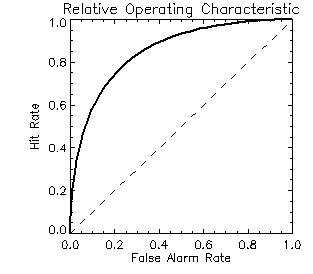
\includegraphics[scale=0.70]{fig/ROC}
\caption{\label{fig:ROC}Receiver operating characteristics curve.  True positive or hit rate is shown as a function of false positive or false alarms rate.  The dashed line shows the ROC curve of the random guess.}
\end{figure}


The ROC curve allows a visual exposition of the family of classifiers $\mathcal{H}$.  In particular, it is easy to see which threshold is needed for a certain hit rate or true positive rate.  Moreover, it is also of interest to reduce all this information into a single number.  The area under the ROC curve, also known as AUC, is such a number.  
AUC is independent of $T$ and also the priors.  It may be difficult to comprehend what AUC is at this point, but we will return to it afterward.

First, let $X_0$ and $X_1$ be random variables with probability distributions $P(X | Y = 0)$ and $P(X | Y = 1)$, respectively.  We define the random variables $Q_0 = q(X_0)$ and $Q_1 = q(X_1)$.  To summarize, $Q_0$ is basically the output value you get when you pick a random sample of class zero. The same thing can be said for $Q_1$.  

The probability $P(Q_1 > Q_0)$ is of interest, because this says what is the probability that if you take one sample by random from each of the populations, what is the chance that the output value from sample one is higher than the output value of sample zero.  This question is independent of $T$, meaning that the discussion about priors and costs are not needed. This probability is called the concordance probability.

Without exposing the details, it is possible to show that
\begin{equation}
\label{eq:concurrent}
\mbox{AUC} = P(Q_1 > Q_0).
\end{equation}
It is important to note that nothing need to be assumed about the probability distributions of $Q_0$ and $Q_1$.  Furthermore, it is worth noting that the concordance probability is exactly equal the common language effect size of the Mann-Whitney $U$ test.  We have therefore chosen to add a section of the Mann-Whitney $U$ test.

\subsubsection{Mann-Whitney $U$ test}
\label{sec:U}

In statistics, the Mann-Whitney $U$ test (also called the Mann-Whitney-Wilcoxon (MWW), Wilcoxon rank-sum test, or Wilcoxon-Mann-Whitney test) is a nonparametric test of the null hypothesis that two populations are the same against an alternative hypothesis, especially that a particular population tends to have larger values than the other.  It has greater efficiency than the $t$-test on non-normal distributions and it is nearly as efficient as the $t$-test on normal distributions.

We define a data set $Z$ with $n$ input-output pairs $(x_i, y_i)$, independently drawn from $P(X,Y)$.  From the data set we have two populations $\bv{q_0} = \{q(x_i) , | \, y_i = 0 \}$ and $\bv{q_1} = \{q(x_i) , | \, y_i = 1 \}$.  Their sizes are $n_0$ and $n_1$ so that $n_0 + n_1 = n$.  Calculating the $U$ statistics is straightforward, where these two values are obtained 

\begin{equation}
\label{eq:U}
U_0 = \sum_{i=1}^{n_0}\sum_{j=1}^{n_1} H(\,q_{1,j} - q_{0,i}    \,) \quad \mbox{and} \quad 
U_1 = \sum_{i=1}^{n_0}\sum_{j=1}^{n_1} H( \,q_{0,i} - q_{1,j}    \,).
\end{equation}
Here, $H(\cdot)$ is the heaviside step function and notice that $U_0 + U_1 = n_0n_1$.  For large samples, each U is approximately normally distributed. In that case, the standardized value

\begin{equation}
\label{eq:z}
z = \frac{U_0 - m_{U}}{\sigma_{U}},
\end{equation}
where $m_U$ and $\sigma_U$ are the mean and standard deviation of $U$ given by

\begin{equation}
\label{eq:z}
m_U = \frac{n_0n_1}{2} \quad \mbox{and} \quad 
\sigma_U = \sqrt{\frac{n_0n_1(n_0 + n_1 + 1)}{12} }.
\end{equation}

Significance of test can be checked in tables of the normal distribution.  Although, such an hypothesis test is interesting by itself, we are more interested in the concordance probability $P(Q_1 > Q_0)$ which is defined by

\begin{equation}
\label{eq:concordance}
P(Q_1 > Q_0) = \frac{U_1}{n_0n_1}.
\end{equation}

It is important to note that even though the Mann-Whitney $U$ test is dependent on wether the shapes of the probability distributions of $Q_0$ and $Q_1$ are similar, this requirement is not necessary for the concordance probability.  Also. equation \eqref{eq:concordance} shows a simple way of calculating $P(Q_1 > Q_0)$ and AUC.

\subsection{Performance measures for classification on streaming data}
\label{sec:stream}

This section includes various evaluation methods for classification on data streams.  Central to choices of evaluation methods are stationarity versus concept-drift, class imbalance, wether a scoring function exist, computational constraints and also the importance of earliness of warnings.

\subsubsection{Stationary data streams}

Let $\{X_{t}\}$ be a stochastic process, where $F_X(\bm{x_{t_1 + \tau}},...,\bm{x_{t_k + \tau}} )$ is the cumulative distribution function of the joint distribution at $t_1 + \tau,...,t_k + \tau$.  Then $\{X_t\}$ is a stationary process, or a stationary stream, if, for all $k$, for all $\tau$ and for all $t_1 + \tau,...,t_k + \tau$, 

\begin{equation}
\label{eq:stationarity}
F_X(\bm{x_{t_1 + \tau}},...,\bm{x_{t_k + \tau}} ) = F_X(\bm{x_{t_1}},...,\bm{x_{t_k}} ),
\end{equation}
where the $\bm{x_t}$s are vectors of fixed size.  Clearly, $F_X(\cdot)$ is not a function of time.  

In stationary streams, the mean and the variance, if they exist, do not vary.  The covariance structures to neighboring instances are also preserved.  To summarize, stationary streams are more general than i.i.d. streams, where the covariance to all other instances are zero.  

In \cite{Gam13}, the prequential empirical risk is defined as 

\begin{equation}
\label{eq:prequentialRisk}
R_{emp}(h, \{X_{t_k}\}) = k^{-1} \sum_{i=1}^k L(\bm{x_{t_i}} , h(\bm{x_{t_i}} ), y_{t_i}),
\end{equation}
where $y_{t_i}$ is the class label at time $t_i$ and $n$ is the number of samples up to $t_k$.  In the original paper, the notation is different and the measure is called the prequental error  Adaptations are made to comply with notation and definitions in section \ref{sec:static}.  Notice, that the loss function in the prequential empirical risk, is generalized compared to \cite{Gam13}, to also include dependency of $\bm{x_{t_i}}$, which may in fact be just $t_i$.  This generalization means that it is possible to model evolving loss as well.

\todo{Include a discussion of statistical interpretation of loss functions on stationary data.  Dependence between timesteps is essential. Is this a problem? What opportunities do we have with evolving loss? Maybe nothing, but worth reflecting on.}

In the case when the classification is based on a scoring function, which is common for Bayesian networks, then the prequential AUC at time step $t_k$ can be calculated by
\begin{equation}
\label{eq:prequentialAUC}
\mbox{AUC}_{t_k}= \frac{U_{1,k}}{n_{0,k}n_{1,k}},
\end{equation}
where $n_{0,k}$ and $n_{1,k}$ are the number of negatives and positives up to $t_k$.  To be precise, $n_{0,k} + n_{1,k} = k$.  The quantity $U_{1,k}$ is calculated by the second $U$-statistic as of equation \eqref{eq:U} (using $n_{0,k}$ and $n_{1,k}$).

On a data stream there is an opportunity of calculating AUC recursively with the following algorithm.

\begin{equation}
\label{eq:prequentialAUC2}
U_{1,k}= 
\begin{cases}
U_{1,k-1} + \sum_{j=1}^{n_{1,k}} H( \,q_{0,n_{0,k}} - q_{1,j}    \,)
 \quad &\mbox{for} \quad y_{t_k} = 0\\
U_{1,k-1} + \sum_{i=1}^{n_{0,k}} H( \,q_{0,i} - q_{1,n_{1,k}}    \,)
\quad &\mbox{for} \quad y_{t_k} = 1.\\
\end{cases}
\end{equation}
Clearly AUC claculation is $O(k)$, which might be a problem for very long streams.  

It is worth noting a few points about the statistical interpretability of AUC on stationary streams.  Unless the stream is also i.i.d. the $q_{0,i}$s and the $q_{1,i}$s are generally dependent on neighboring points.  This fact is however not contradicting the fact that AUC is equal to the concordance probability $ P(Q_1 > Q_0)$.  This is because the definitions of $Q_0$ and $Q_1$ are $Q_0 = q(X_0)$ and $Q_1 = q(X_1)$ and 
that $X_0$ and $X_1$ are random variables with probability distributions $P(X | Y = 0)$ and $P(X | Y = 1)$.  In practice, samples of $Q_0$ and $Q_1$ can be though of as picking samples from $\bv{q_0}$ and $\bv{q_1}$, respectively.

\subsubsection{Data streams that involve concept-drift}

Consept drift is generally understood as unforeseen changes in statistical properties of the target variable.  In the case of regression this can basically be understood as non stationarity of the dependent variable.  In the case of classification, it is understood as the class distribution being \emph{not} constant.  

However, this definition is not always clear cut in the literature.  For instance in \cite{Brz14}, concept drift is understood broader involving changes in explanatory variables and the predictor itself.  \todo{Clarify a bit more.}  For clarity, in this paper we refer to consept drift as changes in the target variable alone.

In \cite{Gam13}, two estimators where suggested for dealing with concept drift and/or non stationary explanatory variables.  The first estimator involves calculating the prequential empirical risk over a sliding window of $w$ samples. 

\begin{equation}
\label{eq:prequentialRisk2}
R_{emp}(t_k, h_k, \{X_{t_k}\}, w) = w^{-1} \sum_{i=k - w +1}^k L(\bm{x_{t_i}} , h_k(\bm{x_{t_i}} ), y_{t_i}).
\end{equation}
Notice that $R_{emp}(t_k, h_k, \{X_{t_k}\}, w)$ is a function of time and not just a single number.  The measure reflects the expected loss as a function of time.  Notice also that the classification rule itself $h_k$ is allowed to be a function of time.

The second estimator involves fading factors and is defined as follows

\begin{equation}
\label{eq:prequentialRisk3}
R_{emp}(t_k, h_k, \{X_{t_k}\}, \alpha) =\frac{\sum_{i=1}^k \alpha^{i-k}L(\bm{x_{t_i}} , h(\bm{x_{t_i}} ), y_{t_i})}{\sum_{i=1}^k \alpha^{i-k}} \quad \mbox{where} \quad 0 \leq \alpha \leq 1.
\end{equation}
When $\alpha$ is equal to one, this reduces to the prequental empirical risk with no forgetting factor, while in the case when $\alpha$ is equal to zero, the estimator reduces to the loss function at $t_k$.

In the special case when the loss function is one when the classification is correct and zero elsewhere and $h$, or $h_k$, is consistent, then it is shown in \cite{Gam13} that $R_{emp}(t_k, h_k, \{X_{t_k}\}, \alpha)$, $R_{emp}(t_k, h_k, \{X_{t_k}\}, w) $ and $R_{emp}(h, \{X_{t_k}\})$ approximates the Bayes error in the limiting cases.

In \cite{Brz14}, the prequantial AUC with a forgetting factor is suggested.  The method involves calculating AUC on a sliding window of fixed size.  In general the method involves keeping a sorted list of scores, together with the labels (positives or negatives).  It also involves keeping track of the number of positives and negatives  \todo{Add details on this algorithm. Some pseudocode would work} 

\todo{Discuss stationary explanatory variables with consept drift versus non stationary explanatory variables with concept drift.}

\todo{Drift detection with prequential AUC and prequential loss}

\subsubsection{Early and late warnings}
Methods or reflections on how to incorporate
The substream method

%
%In the use case scenarios in the Amidst software, all problems are binary classifiers, which involve dividing the streams into sub streams that are labeled as either positives or negatives.  There are two important approaches here.
%
%The first approach deals with multiple streams and the global time dependence is removed by sampling all these streams into multiple sub streams, which are starting and ending at the same time steps.  Each sub stream is labeled as either a positive or negative based on the data at the end time.  An evaluation time step that is a fixed between the start and the end is also defined.  The explanatory variables are derived from the data between the start and the evaluation time step.  In this sense, the data is basically i.i.d.
%
%The second approach is when there is basically one stream where one can assume stationarity on a global scale.  Sub streams with large enough distance to other sub streams are taken out of the stream.  These sub streams are labeled as either a positive or a negative.  For instance, a positive is when something is happening towards the end of the sub stream, while a negative is a sub stream where nothing happens.  When the AMIDST software run, the output function is evaluated at each time step.  Depending of the problem, a heuristic algorithm is chosen to output a single number for each sub stream based on the output values.  This can for instance be the maximum value of the output function on an interval that is prior to an event.  
%





 

%\emph{Here we should cover general methods for doing test and evaluation of models in a streaming
%  context. These methods will subsequently be instantiated in relation to the three use case providers so I
%  guess that we should primarily consider the methods that are directly related to the needs of the use case
%  providers, but (taking the back ground of one of the reviewers into account) we might probably benefit from
%  going a bit beyond the immediate needs and put all this stuff into a broader context ...}
%
%\cite{Kap14}, \cite{Gam09}, \cite{Gam09_2}, \cite{Gam13}, 
